\documentclass[12pt]{article}
\usepackage{graphics}
\usepackage{graphicx}
\usepackage{float}
\title{\textbf{ Introduction to Latex}}
\author{ Hareesh }

\begin{document}

\maketitle
\newpage

\tableofcontents
\newpage


\section {About Latex}
\textbf{ LaTeX }  is a word processor and document markup language. It is distin-
guished from typical word processors such as Microsoft Word and Apple
Pages in that the writer uses plain text as opposed to formatted text, relying
on markup tagging conventions to define the general structure of a document
(such as article, book, and letter), to stylise text throughout a document
(such as \textbf{ bold } and \textit{italic}), and to add citations and cross-referencing. A \textbf{TeX}
distribution such as \textbf{TeXlive} or \textbf{MikTeX} is used to produce an output file
(such as PDF or DVI) suitable for printing or digital distribution.\\

\textbf{LaTeX} is used for the communication and publication of scientific doc-
uments in many fields, including mathematics, physics, computer science,
statistics, economics, and political science.It also has a prominent role in
the preparation and publication of books and articles that contain complex
multilingual materials, such as Sanskrit and Arabic. \textbf{LaTeX} uses the \textbf{TeX}
typesetting program for formatting its output, and is itself written in the
\textbf{TeX} macro language.\\

\textbf{LaTeX} is widely used in academia. \textbf{LaTeX} can be used as a standalone
document preparation system, or as an intermediate format. In the lat-
ter role, for example, it is often used as part of a pipeline for translating
DocBook and other XML-based formats to PDF. The typesetting system
offers programmable desktop publishing features and extensive facilities for
automating most aspects of typesetting and desktop publishing, including
numbering and cross-referencing of tables and figures, chapter and section
headings, the inclusion of graphics, page layout, indexing and bibliographies.\\

Like \textbf{TeX}, \textbf{LaTeX} started as a writing tool for mathematicians and com-
puter scientists, but from early in its development it has also been taken
up by scholars who needed to write documents that include complex math
expressions or non-Latin scripts, such as Arabic, Sanskrit and Chinese.\\

\textbf{LaTeX} is intended to provide a high-level language that accesses the
power of \textbf{TeX}. LaTeX comprises a collection of TeX macros and a pro-
gram to process \textbf{LaTeX} documents. Because the plain \textbf{TeX} formatting
commands are elementary, it provides authors with ready-made commands
for formatting and layout requirements such as chapter headings, footnotes,
for formatting and layout requirements such as chapter headings, footnotes,
cross-references and bibliographies.\\

\textbf{LaTeX} was originally written in the early 1980s by \textbf{Leslie Lamport} at
SRI International. The current version is LaTeX2e. \textbf{LaTeX} is free software
and is distributed under the \textbf{LaTeX} Project Public License (LPPL) \textbf{(Source
Wikipedia)}.

\section{Opening and Compiling Tex Document}

First create a \textbf{.tex }file using text editor such as \textbf{Vi} or \textbf{Gedit} or \textbf{Kile}.
\subsection{Starting and Ending} \label{two}

A minimal input file looks like following\\


\indent {\textbf{\textbackslash documentclass\{class\}\\
\indent \textbackslash begin\{document\}\\
\indent \indent your text...\\
\indent \textbackslash end \{document\} }\\

where the class is a valid document class for \textbf{ LaTeX}.

\subsection{Compiling the LaTeX Document}

We open the terminal and go to the directory in which our \textbf{ .tex} file is stored
and the we execute the command\\

\textbf{ pdflatex example.tex }\\

\newpage
\section {Section}
Sectioning commands provide the means to structure your text into units:\\\\
\textbf{\textbackslash part \\\\
\textbackslash chapter \\\\
(report and book class only)\\\\
\textbackslash section\\\\
\textbackslash subsection\\\\
\textbackslash subsubsection\\\\
\textbackslash paragraph\\\\
\textbackslash subparagraph}\\\\
All sectioning commands take the same general form, e.g.,\\


\textbf {\textbackslash chapter[toctitle]\{title\}\\}


In addition to providing the heading title in the main text, the section
title can appear in two other places:\\
\begin{enumerate}
 \item The table of contents.
 \item The running head at the top of the page.
\end{enumerate}

You may not want the same text in these places as in the main text. To
handle this, the sectioning commands have an optional argument \textbf{toctitle}
that, when given, specifies the text for these other places.\\

Also, all sectioning commands have *-forms that print title as usual, but
do not include a number and do not make an entry in the table of contents.\\\\
For instance:\\\\
\indent \textbf {\textbackslash section*\{Preamble\}}\\\\
\indent The\textbf{ \textbackslash appendix }command changes the way following sectional units are
numbered. The\textbf{ \textbackslash appendix }command itself generates no text and does not
affect the numbering of parts.\\\\
The normal use of this command is something like\\


\indent \textbf{\textbackslash chapter{A Chapter}\\
\indent ...\\
\indent \textbackslash appendix\\
\indent \textbackslash chapter{The First Appendix}}\\ 


\indent The secnumdepth counter controls printing of section numbers. The set-
ting suppresses heading numbers at any depth \textgreater  level, where chapter is level
zero.\\


\indent \textbf {\textbackslash setcounter\{secnumdepth\}\{level\} }\\


\section{Cross Reference}
One reason for numbering things like figures and equations is to refer the
reader to them, as in \textquotedblleft Figure 3 for more details.\textquotedblright

\subsection{\textbackslash label\{key\} }
A   \textbf{\textbackslash label} command appearing in ordinary text assigns to key the number
of the current sectional unit; one appearing inside a numbered environment
assigns that number to key.\\


A key name can consist of any sequence of letters, digits, or punctuation
characters. Upper and lowercase letters are distinguished.\\


To avoid accidentally creating two labels with the same name, it is com-
mon to use labels consisting of a prefix and a suffix separated by a colon or
period. Some conventionally-used prefixes:\\\\
\textbf{ch}  \indent for chapter\\
\textbf{sec}\indent for lower-level sectioning commands\\
\textbf{fig} \indent for figures\\
\textbf{tab}\indent for tables\\
\textbf{eq}   \indent for equations\\


\subsection{\textbackslash pageref\{key\} }
The \textbf{\textbackslash pageref \{ key \} } command produces the page number of the place in
the text where the corresponding \textbf{\textbackslash label \{ key \} } command appears.


\subsection{\textbackslash ref\{key\} }
The \textbf{\textbackslash ref } command produces the number of the sectional unit, equation,
footnote, figure, . . . , of the corresponding \textbf{\textbackslash label} command. It does not
produce any text, such as the word \textquoteleft Section\textquoteright or \textquoteleft Figure\textquoteright, just the bare number
itself.


\section{Fonts}

\subsection{Font Styles}
A few of the font styles which are useful are listed below
\begin{enumerate} 
\item \textrm{\textbackslash textrm (Roman)}
\item \textit{\textbackslash textit (Italics)}
\item \textbf{\textbackslash textbf (Bold)}
\item \emph{\textbackslash emph (Emphasis)}
\item \texttt{ \textbackslash texttt (Typewriter)}
\item \textnormal{ \textbackslash textnormal (Normal font)}
\end{enumerate}
Example to output text in bold we can type\\\\ 
\textbf{\textbackslash textbf\{anything you type inside the curly braces will be outputed
in bold\} }\\
\subsection{Font Sizes}
The following standard type size commands are supported by \textbf{ LaTeX}.

\begin{table}[H]
\caption{Font Sizes}
\centering
\begin{tabular} {l|c|c|c}

\hline
{Command} & {10pt} & {11pt}  & {12pt}\\ \hline \hline
\tiny \textbackslash tiny  & 5 & 6 & 6 \\
\scriptsize \textbackslash scriptsize & 7 & 8 & 9 \\
\footnotesize \textbackslash footnotesize & 9 & 10 & 10.95 \\
\small \textbackslash small & 10 & 10.95 & 12 \\
\textbackslash normalize(default)& 12 & 12 & 14.28\\
\large \textbackslash large & 14.4 & 14.4 & 17.28\\
\LARGE \textbackslash LARGE & 17.28 & 17.28 & 20.74\\
\huge \textbackslash huge & 20.74 & 20.74 & 24.88\\
\Huge \textbackslash Huge & 24.88 & 24.88 & 24.88\\
\hline
\end{tabular}
\end{table}

The commands as listed here are declaration forms. The scope of the
declaration form lasts until the next type style command or the end of the
current group.\\



\section{Images}
To insert an image we first need to include a package called \textbf{graphicx} after
the documentclass as mentioned in section \ref{two}. To insert the image into the
PDF we have to use the following commands\\\\\\
\textbf{\textbackslash begin\{figure\}[h]\\
\textbackslash centering\\
\textbackslash caption\{Example Picture Created Using Dia\}\\
\textbackslash includegraphics[scale=0.7] \{img.png\}\\
\textbackslash end\{figure\} }\\\\
Figures are objects that are not part of the normal text, and are instead
floated to a convenient place, such as the top of a page. Figures will not be
split between two pages.\\

\begin{figure}[h]
\centering
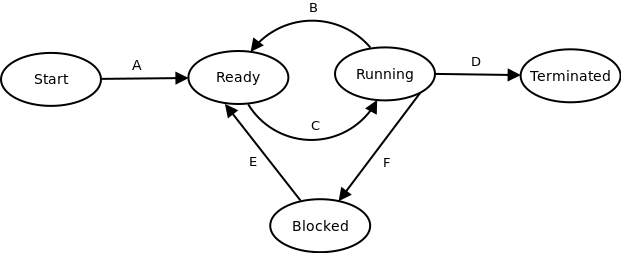
\includegraphics[scale=0.5] {OS.png}
\caption{Example Picture Created Using Dia}
\end{figure}

\section{Tables}
\subsection{ Multi Row Tables}
To combine rows the package multirow must be imported with\\
in your preamble, then you can use the \textbf{ \textbackslash multirow} command in your docu-
ment:\\
\textbf{\textbackslash usepackage\{multirow\} }\\\\
The table below includes mathematical notations, which you can produce
by embedding the experession in  \textdollar  \textdollar   delimiters. For subscript, use underscore
and for superscript, use carrot.\\


\begin{table}
\caption{Example of Multi Row Table}
\centering
\begin{tabular} {|l|  p{6cm} |}
\hline
{\textbf {Algorithms}} & {\textbf{Time Complexity}} \\ \hline \hline
 {Bubble Sort} & 
 Best Case : O(n)
\newline Average Case : O(\textit {n\textsuperscript2})
\newline Worst Case : O(\textit{n\textsuperscript2})\\
\hline
\hline
Merge Sort & 
Best Case : O(\textit{n log\textsubscript2(n)}) 
\newline Average Case : O(\textit{n log\textsubscript2(n)})
\newline Worst Case : O(\textit{n log\textsubscript2(n)}) \\
\hline
\hline
Quick Sort & 
Best Case : O(\textit{n log\textsubscript2(n)})
\newline Average Case : O(\textit{n log\textsubscript2(n)})
\newline Worst Case : O(\textit{n\textsuperscript2})  \\
\hline
\hline

\end{tabular}
\end{table}

\subsection{Table of Figures}


\begin{table}[H]
\caption{Example of Table of Figures}
\centering
\begin{tabular} {c c}

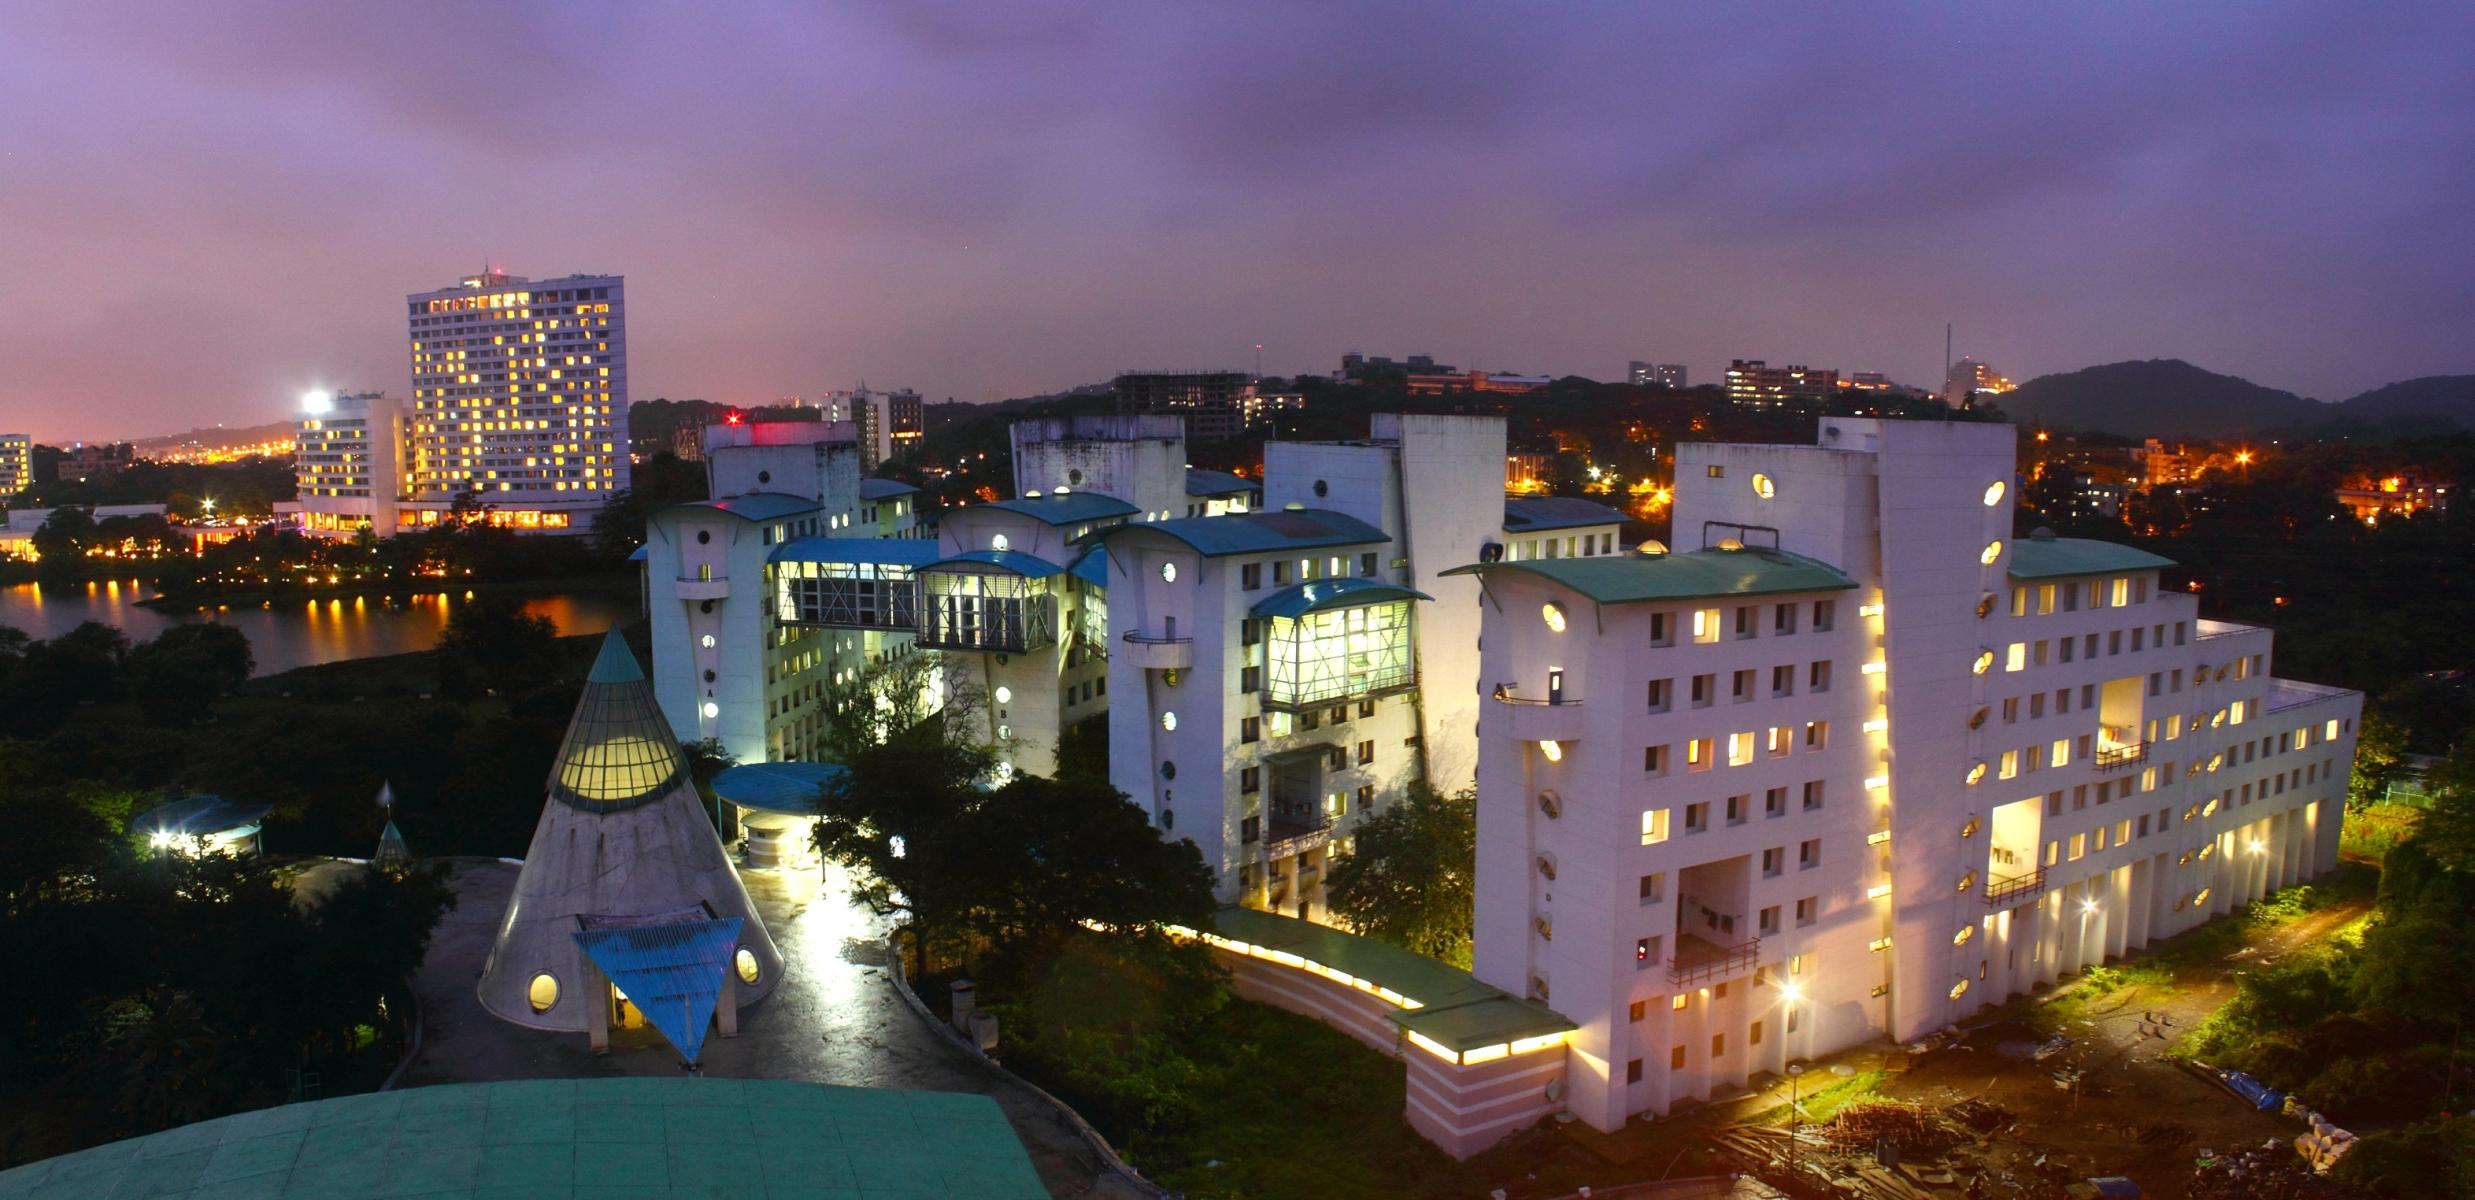
\includegraphics[width=6cm,height=3.5cm]{1.jpeg}
   & 
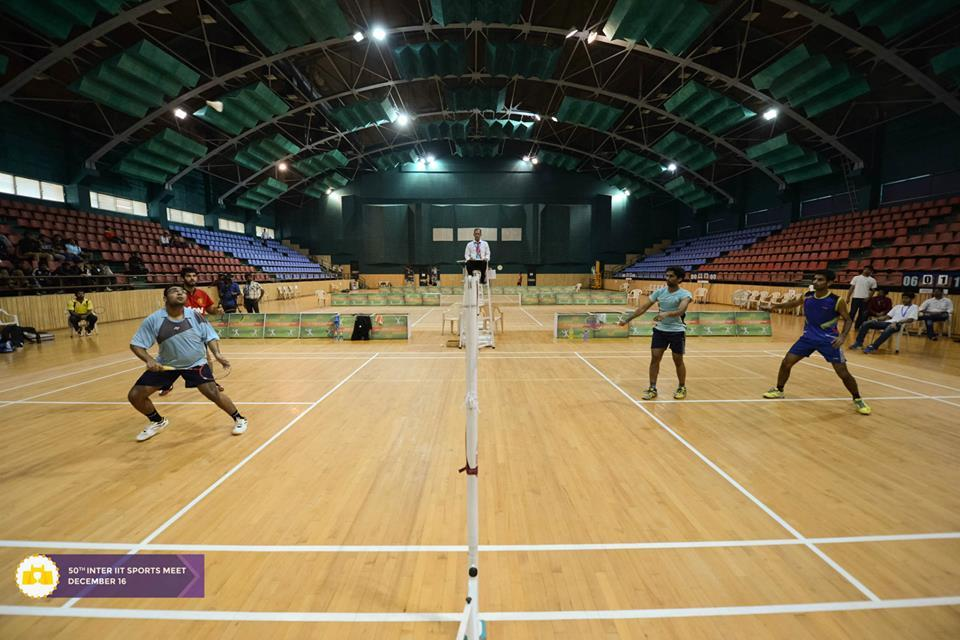
\includegraphics[width=6cm,height=3.5cm]{2.jpeg}\\

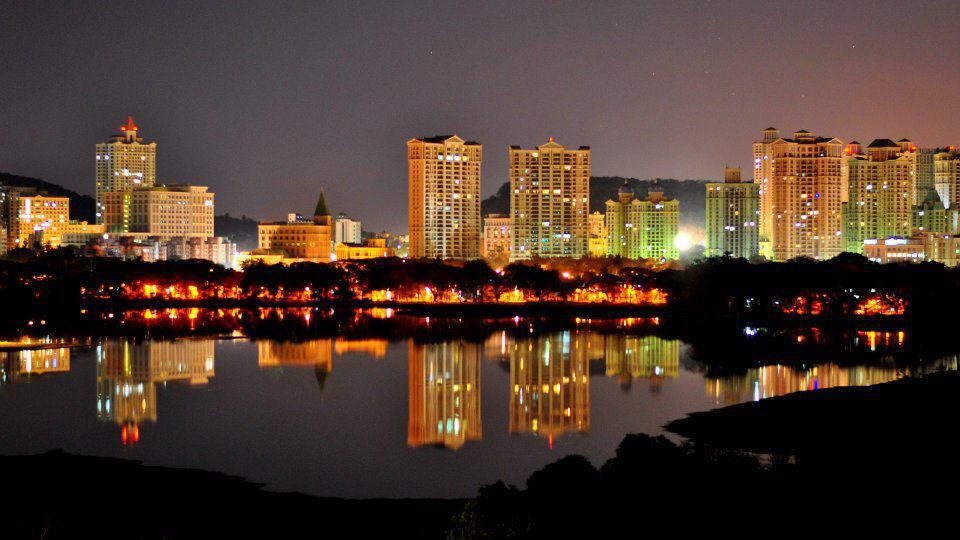
\includegraphics[width=6cm,height=3.5cm]{3.jpeg}
   & 
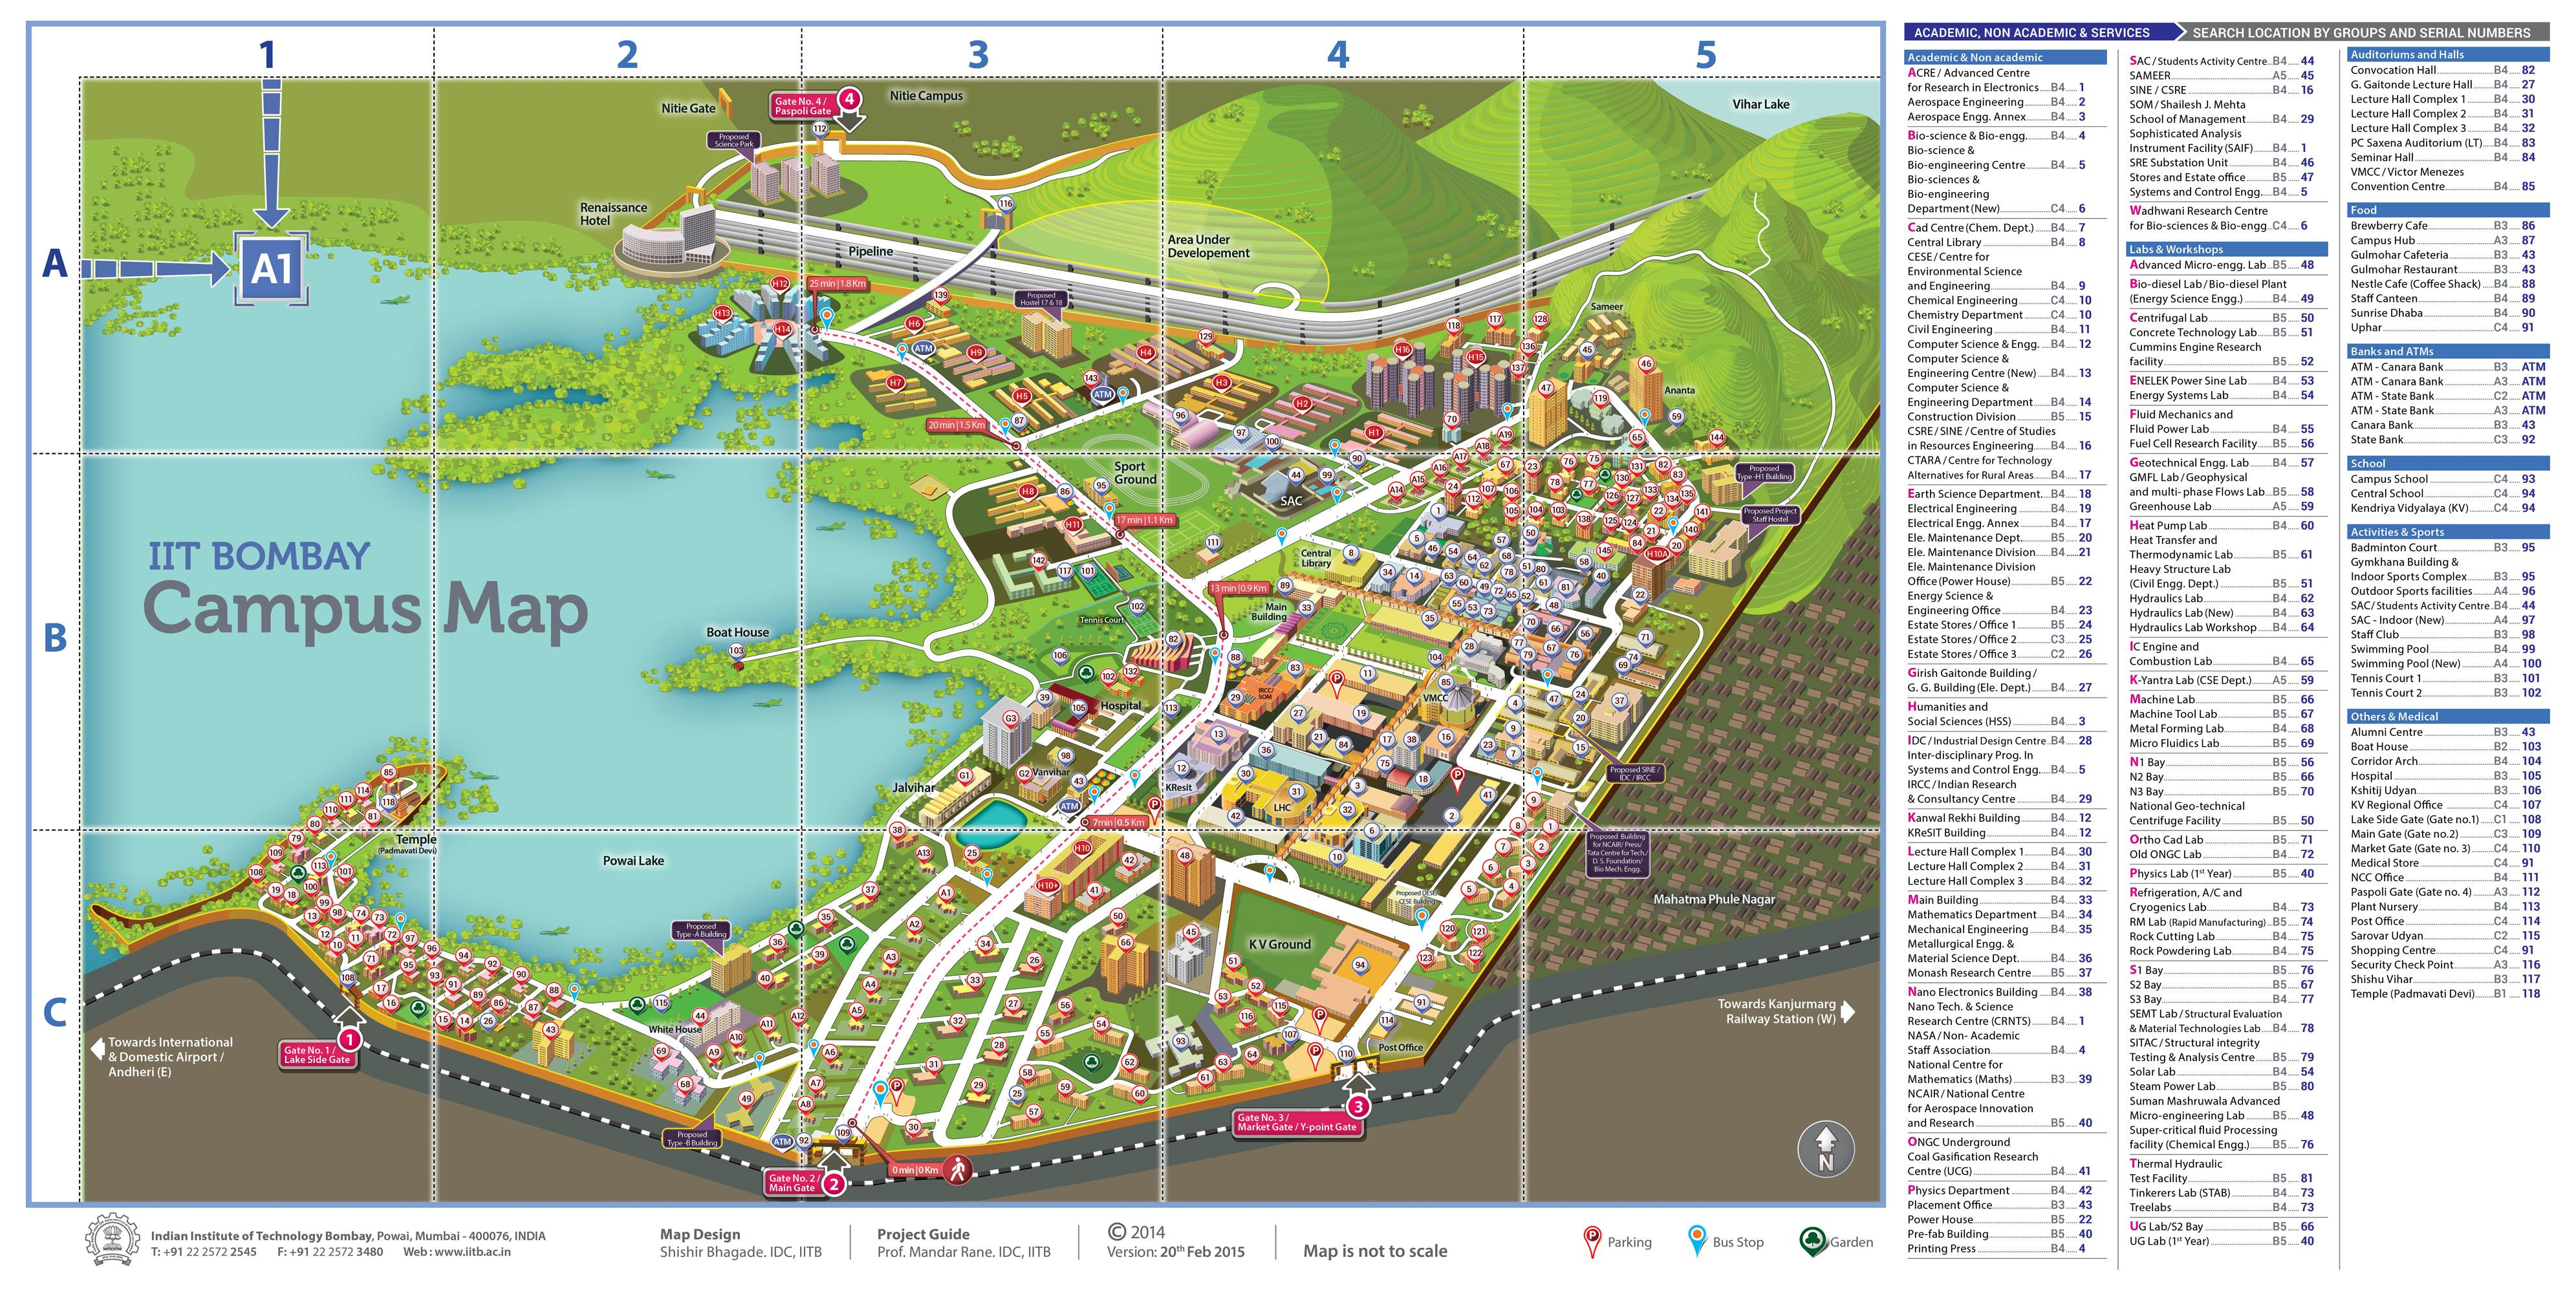
\includegraphics[width=6cm,height=3.5cm]{4.jpeg}\\
\end{tabular}
\end{table}

\newpage
\section{Conclusion}
Thus by using \textbf{LaTeX} we can create reports, articles etc on the fly without
worrying about the alignment, typeset etc making it very productive.\textbf{LaTeX}
has become a popular tools among students, teachers, research scholars etc
as it is a free software available on any Linux platform.


\end{document}
